\documentclass[10pt,landscape,a4paper]{article}
\usepackage[utf8]{inputenc}
\usepackage[ngerman]{babel}
\usepackage{tikz}
\usetikzlibrary{shapes, positioning, arrows, fit, calc, graphs, graphs.standard}
\usepackage[nosf]{kpfonts}
\usepackage[t1]{sourcesanspro}
%\usepackage[margin=0.05in]{geometry}
%\usepackage[lf]{MyriadPro}
%\usepackage[lf,minionint]{MinionPro}
\usepackage{multicol}
\usepackage{wrapfig}
\usepackage[top=0.2mm,bottom=2mm,left=1mm,right=1mm]{geometry}
\usepackage[framemethod=tikz]{mdframed}
\usepackage{microtype}
\usepackage{bbold}
\usepackage{wrapfig}
\usepackage{dsfont} % For mathbb{1}
\usepackage{amsmath}

% START CHEATSHEET TEMPLATE

\usepackage[default]{raleway}
\usepackage{fontawesome}
\usepackage[T1]{fontenc}

\usepackage{hyperref}
\usepackage{enumitem}
\setlist[enumerate]{itemsep=0mm}
\usepackage{lipsum}

\usepackage{xcolor}
\definecolor{customcolor}{HTML}{b5e9ff}
\definecolor{alert}{HTML}{CD5C5C}
\definecolor{w3schools}{HTML}{4CAF50}
\definecolor{subbox}{gray}{0.60}
\definecolor{codecolor}{HTML}{000000}
\colorlet{xx}{customcolor}

\usepackage{paralist}


%--------------------------Editor mode.

\usepackage
[citestyle=authoryear,
sorting=nty,	  		%Sorts bibliography by year, name, title
autocite=footnote, 		%Autocite command generates footnotes
autolang=hyphen, 		
mincrossrefs=1, 	
backend=biber]
{biblatex}

\DeclareFieldFormat{postnote}{#1}
\DeclareFieldFormat{multipostnote}{#1}
\DeclareAutoCiteCommand{footnote}[f]{\footcite}{\footcites}

\bibliography{literature}
%----------------------------------------
%--------------------------------------------------------------------------------
\usepackage{tcolorbox}

\tcbuselibrary{most, listingsutf8, minted}

\tcbset{tcbox width=auto,left=1mm,top=1mm,bottom=1mm,
right=1mm,boxsep=1mm,middle=1pt}

\newenvironment{mycolorbox}[2]{%
\begin{tcolorbox}[grow to left by=-1em,grow to right by=-1em,capture=minipage,fonttitle=\large\bfseries, enhanced jigsaw,boxsep=1mm,colback=#1!30!white,on line,tcbox width=auto, toptitle=0mm,colframe=#1,opacityback=0.7,nobeforeafter,title=#2]%
}{\end{tcolorbox}\\[0.2em]}

\newenvironment{subbox}[2]{%
\begin{tcolorbox}[capture=minipage,fonttitle=\normalsize\bfseries, enhanced jigsaw,boxsep=1mm,colback=#1!30!white,on line,tcbox width=auto,left=0.3em,top=1mm, toptitle=0mm,colframe=#1,opacityback=0.7,nobeforeafter,title=#2]\footnotesize %
}{\normalsize\end{tcolorbox}\vspace{0.1em}}

\newenvironment{multibox}[1]{%
\begin{tcbraster}[raster columns=#1,raster equal height,nobeforeafter,raster column skip=1em,raster left skip=1em,raster right skip=1em]}{\end{tcbraster}}

\newenvironment{textbox}[1]{\begin{mycolorbox}{customcolor}{#1}}{\end{mycolorbox}}

%-------------------------------
\newtcblisting{codebox}[2]{colback=codecolor!5,colframe=codecolor!80!black,listing only, 
minted options={numbers=left,style=tcblatex,fontsize=\scriptsize,breaklines,autogobble,linenos=false,numbersep=2mm},
left=4mm,enhanced,boxsep=1pt,left=2pt,right=1pt,top=0pt,bottom=0pt,
title=#2, fonttitle=\bfseries,
listing engine=minted,minted language=#1}

%--------------------------------------------------------------------------------
\newcommand{\punkti}{~\lbrack\dots\rbrack~}

\renewenvironment{quote}
               {\list{\faQuoteLeft\phantom{ }}{\rightmargin\leftmargin}%
                \item\relax\scriptsize\ignorespaces}
               {\unskip\unskip\phantom{xx}\faQuoteRight\endlist}
               

%--------------------------------------------------------------------------------
\newcommand{\bgupper}[3]{\colorbox{#1}{\color{#2}\huge\bfseries\MakeUppercase{#3}}}
\newcommand{\bg}[3]{\colorbox{#1}{\bfseries\color{#2}#3}}

\newcommand{\mycommand}[2]{{\ttfamily\detokenize{#1}}~\dotfill{}~{\footnotesize #2}\\}
\newcommand{\sep}{{\scriptsize~\faCircle{ }~}}


\newcommand{\bggreen}[1]{\medskip\bgupper{w3schools}{black}{#1}\\[0.5em]}
\newcommand{\green}[1]{\smallskip\bg{w3schools}{white}{#1}\\}
\newcommand{\red}[1]{\smallskip\bg{alert}{white}{#1}\\}
\newcommand{\E}{\mathbb{E}}

\makeatletter
\newcommand*\bigcdot{\mathpalette\bigcdot@{.5}}
\newcommand*\bigcdot@[2]{\mathbin{\vcenter{\hbox{\scalebox{#2}{$\m@th#1\bullet$}}}}}
\makeatother

\usepackage{multicol}
\setlength{\columnsep}{4pt}

\setlength{\parindent}{0pt}
\pagestyle{empty}

\usepackage{csquotes}

\newcommand{\loremipsum}{Lorem ipsum dolor sit amet.}

% END CHEATSHEET TEMPLATE

\let\bar\overline

\definecolor{myblue}{cmyk}{1,.72,0,.38}

\def\firstcircle{(0,0) circle (1.5cm)}
\def\secondcircle{(0:2cm) circle (1.5cm)}

\colorlet{circle edge}{myblue}
\colorlet{circle area}{myblue!5}

\tikzset{filled/.style={fill=circle area, draw=circle edge, thick},
    outline/.style={draw=circle edge, thick}}

\pgfdeclarelayer{background}
\pgfsetlayers{background, main}

\everymath\expandafter{\the\everymath \color{myblue}}
\everydisplay\expandafter{\the\everydisplay \color{myblue}}

\renewcommand{\baselinestretch}{.8}
\pagestyle{empty}




\makeatletter
\renewcommand{\section}{\@startsection{section}{0}{0mm}%
                                {0ex}%
                                {0ex}%x
                                {\color{myblue}\sffamily\small\bfseries}}
\renewcommand{\subsection}{\@startsection{subsection}{1}{0mm}%
                                {0ex}%
                                {0ex}%x
                                {\sffamily\bfseries}}
\makeatother

\def\multi@column@out{%
   \ifnum\outputpenalty <-\@M
   \speci@ls \else
   \ifvoid\colbreak@box\else
     \mult@info\@ne{Re-adding forced
               break(s) for splitting}%
     \setbox\@cclv\vbox{%
        \unvbox\colbreak@box
        \penalty-\@Mv\unvbox\@cclv}%
   \fi
   \splittopskip\topskip
   \splitmaxdepth\maxdepth
   \dimen@\@colroom
   \divide\skip\footins\col@number
   \ifvoid\footins \else
      \leave@mult@footins
   \fi
   \let\ifshr@kingsaved\ifshr@king
   \ifvbox \@kludgeins
     \advance \dimen@ -\ht\@kludgeins
     \ifdim \wd\@kludgeins>\z@
        \shr@nkingtrue
     \fi
   \fi
   \process@cols\mult@gfirstbox{%
%%%%% START CHANGE
\ifnum\count@=\numexpr\mult@rightbox+2\relax
          \setbox\count@\vsplit\@cclv to \dimexpr \dimen@-1cm\relax
\setbox\count@\vbox to \dimen@{\vbox to 1cm{\header}\unvbox\count@\vss}%
\else
      \setbox\count@\vsplit\@cclv to \dimen@
\fi
%%%%% END CHANGE
            \set@keptmarks
            \setbox\count@
                 \vbox to\dimen@
                  {\unvbox\count@
                   \remove@discardable@items
                   \ifshr@nking\vfill\fi}%
           }%
   \setbox\mult@rightbox
       \vsplit\@cclv to\dimen@
   \set@keptmarks
   \setbox\mult@rightbox\vbox to\dimen@
          {\unvbox\mult@rightbox
           \remove@discardable@items
           \ifshr@nking\vfill\fi}%
   \let\ifshr@king\ifshr@kingsaved
   \ifvoid\@cclv \else
       \unvbox\@cclv
       \ifnum\outputpenalty=\@M
       \else
          \penalty\outputpenalty
       \fi
       \ifvoid\footins\else
         \PackageWarning{multicol}%
          {I moved some lines to
           the next page.\MessageBreak
           Footnotes on page
           \thepage\space might be wrong}%
       \fi
       \ifnum \c@tracingmulticols>\thr@@
                    \hrule\allowbreak \fi
   \fi
   \ifx\@empty\kept@firstmark
      \let\firstmark\kept@topmark
      \let\botmark\kept@topmark
   \else
      \let\firstmark\kept@firstmark
      \let\botmark\kept@botmark
   \fi
   \let\topmark\kept@topmark
   \mult@info\tw@
        {Use kept top mark:\MessageBreak
          \meaning\kept@topmark
         \MessageBreak
         Use kept first mark:\MessageBreak
          \meaning\kept@firstmark
        \MessageBreak
         Use kept bot mark:\MessageBreak
          \meaning\kept@botmark
        \MessageBreak
         Produce first mark:\MessageBreak
          \meaning\firstmark
        \MessageBreak
        Produce bot mark:\MessageBreak
          \meaning\botmark
         \@gobbletwo}%
   \setbox\@cclv\vbox{\unvbox\partial@page
                      \page@sofar}%
   \@makecol\@outputpage
     \global\let\kept@topmark\botmark
     \global\let\kept@firstmark\@empty
     \global\let\kept@botmark\@empty
     \mult@info\tw@
        {(Re)Init top mark:\MessageBreak
         \meaning\kept@topmark
         \@gobbletwo}%
   \global\@colroom\@colht
   \global \@mparbottom \z@
   \process@deferreds
   \@whilesw\if@fcolmade\fi{\@outputpage
      \global\@colroom\@colht
      \process@deferreds}%
   \mult@info\@ne
     {Colroom:\MessageBreak
      \the\@colht\space
              after float space removed
              = \the\@colroom \@gobble}%
    \set@mult@vsize \global
  \fi}

\makeatother
\setlength{\parindent}{0pt}


\begin{document}
\begin{multicols*}{4}
\scriptsize
\section*{Linear Regression}\; Ass. $Y=X\theta+\epsilon$, $\E[\epsilon]=0$, $\E[\epsilon\epsilon^{\top}]=\sigma^2I_n$
\\
$\cdot\; \E[\epsilon_i^2]\neq0\rightarrow$ weigh. LS $\cdot\; \text{Cov}(\epsilon_i,\epsilon_j)\neq0\rightarrow$ gen. LS $\cdot\; \epsilon\nsim\mathcal{N}\rightarrow$ rob. reg. 
\textbf{LSE}
$\hat \beta = \text{argmin}_\beta ||Y-Xb||_2^2 = (X^\top X)^{-1}X^\top Y$, $\text{Cov}(\hat{\beta})=\sigma^2(X^{\top}X)^{-1}$, $\E[\hat{\beta}]=\beta$,
$\cdot\; \epsilon \sim \mathcal{N}(0,\sigma^2 I)\Rightarrow Y, \hat{\beta}, \hat{Y}, r \sim \mathcal{N}$ and $\hat{\sigma}^2\sim\frac{\sigma^2}{n-p}\chi^2_{n-p}$, where $\hat \sigma^2 = \frac 1 {n-p}RSS$ (unbiased) and $RSS=||Y-X\hat \beta||_2^2=\sum r_i^2$ \\
\textbf{Geometry}: $\hat{Y}=PY$, $r^{\top}x^{(j)}=0\Rightarrow r^{\top}\hat{Y}=0$, $r\in\text{col}(X)^{\perp}$\\
\textbf{Gen LS}: $\Sigma$ known/$\sigma^2G$ w $\sigma$ unknown $\rightarrow$ $\Sigma=CC^{\top}$ (e.g. Cholesky $C\in \nabla-$lower)
$\tilde{Y}=C^{-1}Y=C^{-1}X\beta+C^{-1}\epsilon=\tilde{X}\beta+\tilde{\epsilon}$ $\rightarrow$
$\hat \beta =  (X^{\top} \Sigma^{-1} X)^{-1} X^{\top} \Sigma^{-1} Y$ and $\text{Cov}(\beta)=(X^T\Sigma^{-1}X)^{-1}$\\
$\Sigma=\sigma^2\text{diag}(z_1,\dots,z_n) \rightarrow $ weightLS $\arg\min_{\theta} \sum z_i^{-1} (y_i-x_i^{\top}\theta)^2$
\begin{codebox}{r}{Linear Regression}
fit <- lm(y~x1+x2) # Fit only x1 and x2 (so p=3)
predict(fit, pred.data.frame)
# Manual fit
X <- cbind(1, x1, x2) # p = 3
XtX.inv <- solve(t(X) %*% X)
beta.hat <- XtX.inv %*% t(X.int) %*% y
res <- y - X.int %*% beta.hat # Residuals
RSE <- sqrt(sum(res^2)/(n-p)) #Resid.std.err.=hat(sd)
se.x1 <- RSE * sqrt(XtX.inv[2, 2]) # Std. error of x1
t.val.x1 <- beta.hat[2] / se.x1 # T value of x1
p.val.x1 <- 2*pt(abs(t.val.x1), df=n-p, lower=F)
# Alternative t-value
coef <- summary(fit1)$coefficients
t1 <- coef["x1","Estimate"]/coef["x1","Std. Error"]
# Poly regression
lm(wage~poly(age,4)) # Orthogonal polynomials
lm(wage~poly(age, 4, raw=T)) # Monomial basis
lm(wage~age+I(age^2)+I(age^3)+I(age^4)) # Alternative
summary(y-model\$fitted.values) # Residuals
\end{codebox}

\subsection*{Tests and model selection}
\textbf{Entry-wise test}\\
$H_0: y = X\beta + \epsilon$ with $\beta_j=0$
$H_A: y = X\beta + \epsilon$ with $\beta_j\neq 0$\\
$\frac{\hat \beta_j - \beta_j}{\sqrt{\sigma^2(X^\top X)^{-1}_{jj}}} \sim \mathcal{N}(0,1)$ $\Rightarrow$
t-statistic: $T_j:=\frac{\hat \beta_j}{\sqrt{\hat \sigma^2 (X^\top X)^{-1}_{jj}}} \stackrel{H_0}{\sim} t_{n-p}$\\
\textbf{P-Value}$=P_{H_0}(T>|t|)$, $t=$ obs. instance of $T$.
If $< \alpha$ then reject $H_0$.
\textbf{ANOVA (Analysis of variance)} $\Vert Y-\bar Y \Vert^2=\Vert  \hat Y - \bar Y\Vert^2+\Vert Y-\hat Y\Vert^2$\\
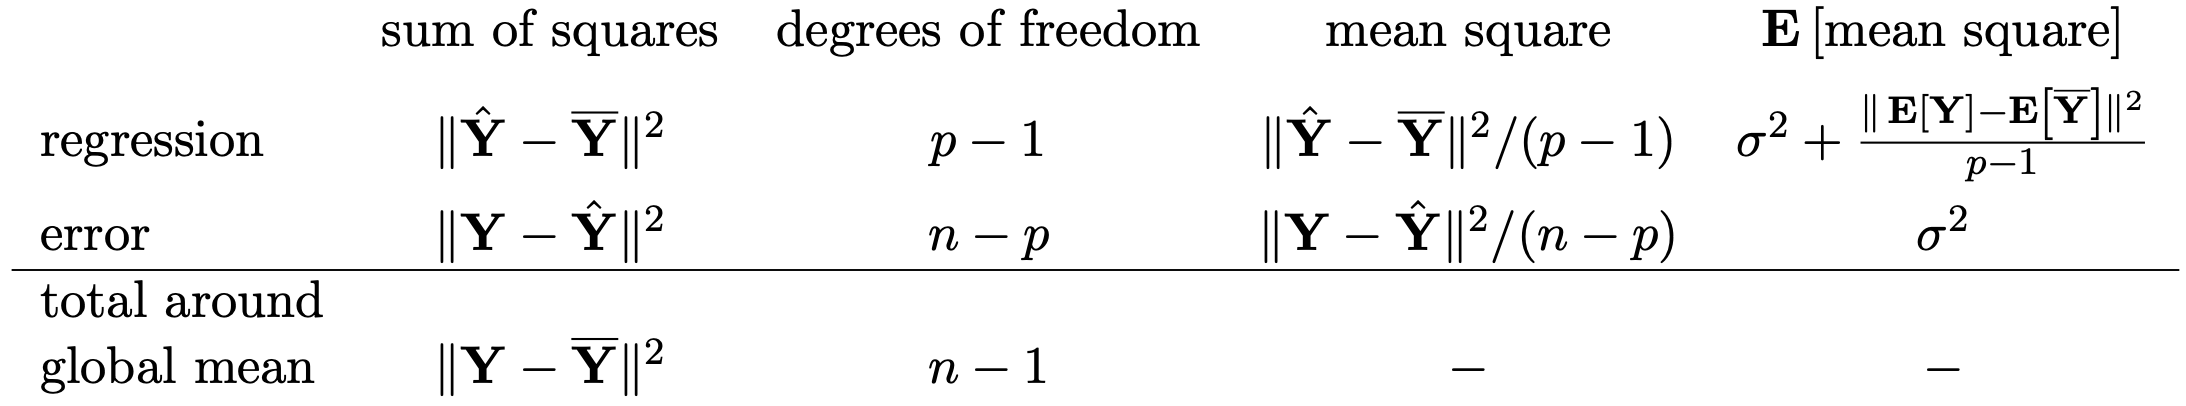
\includegraphics[width = 7cm]{ANOVA.png}
$MSE/\hat{\sigma}^2\rightarrow(H_0:\beta = 0) \Rightarrow F=\frac{\Vert  \hat Y - \bar Y\Vert^2/(p-1)}{\Vert Y- \hat Y\Vert^2/(n-p)}\sim F_{p-1,n-p}$

\begin{codebox}{r}{P-Values \& ANOVA}
fit.smaller <- lm(y ~ x1)
# Anova uses RSS and DoF of largest (last) model, so
# use ascending order!
anova(fit.smaller, fit, fit.all)
# Overall F-Test
fit.empty <- lm(y ~ 1, data=...) # Empty model
anova(fit.empty, fit) # Compare models
# Alternative F-test
Ftest <- summary(fit)$fstatistic
pval <- 1 - pf(Ftest[1], df1=Ftest[2], df2=Ftest[3])
\end{codebox}

BS Alt.: $p=\text{mean}(\#\{\text{m'}:\text{MSE[m'(permuted}[Y],X)] >\text{MSE(m}[Y,X)]\})$

\textbf{R\textsuperscript{2} (Coefficient of determination):} the proportion of the total variation of the response $Y$ around its mean $\bar{Y}$ that is explained by the regression $\hat{Y}$ (via the ANalysis Of VAriance decomposition)
$R^2=\frac{||\hat{Y}-\bar{Y}||^2}{||Y-\bar{Y}||^2}=1-\frac{||Y-\hat{Y}||^2}{||Y-\bar{Y}||^2} = \frac{ESS}{TSS} = 1-\frac{RSS}{TSS}$

\begin{codebox}{r}{R squared}
RSE <- sqrt(sum(residuals(fit)^2)/(n-p))
RSS <- sum(res^2) # Residual sum of squares
TSS <- sum((y - mean(y))^2) # Total sum of squares
R.sq <- 1 - RSS / TSS
AdjR2 <- 1 - (RSS/(n-p))/(TSS/(n-1))
\end{codebox}

\subsection*{Model selection$\;\;$}

BV Tradeoff:
$n^{-1}\sum_{i=1}^n\mathbb{E} \left[ \left( \sum_{j=1}^q \hat{\beta}_j x_{i,j} - m(x_i) \right) ^2 \right]$
$=  n^{-1} \sum_{i=1}^n \left( \mathbb{E}[\sum_{j=1}^q\hat{\beta}_j x_{i, j}] - m(x) \right)^2 + n^{-1}\sum_i \text{Var}(\sum_j \hat{\beta}_j x_{ij})$ and
$n^{-1}\sum_i \text{Var}(\sum_j \hat{\beta}_j x_{ij})=\frac{q}{n} \sigma^2$
\\
Penalized RSS: $||Y - X\beta||^2_2 + \lambda ||\beta||_0$;
\textbf{$\lambda$-choice}: AIC (equiv to $C_p$ for lin Gauss models) $\rightarrow \lambda=2\hat{\sigma}^2$; BIC $\rightarrow \lambda=\log(n)\hat{\sigma}^2$; $\lambda$ by CV
\\
\textbf{Forward Selection:} 1) Fit $M_0$ 2) For $k=0,...,p-1$ fit all $p-k$ models with 1 additional predictor and select best (smallest RSS): $M_k$. 3) Select best among $M_0,....,M_p$ using CV or penalized RSS. \\
\textbf{Backward Selection:} 1) Fit $M_p$ (full model). 2) For $k=p,p-1,...,1$: fit all $k$ models that drop one perdictor in $M_k$. Choose best (smallest RSS): $M_{k-1}$. 3) Select best among $M_0,...,M_p$ using CV or penalized RSS.
\begin{codebox}{r}{Stepwise methods}
library(leaps)
# Try all the submodels
regfit.full=regsubsets(Salary~., data=..., nvmax=19)
# Forward stepwise (method="backward" for backward)
regfit.full=regsubsets(Salary~., data=..., nvmax=19, method="forward")
\end{codebox}

\subsection*{R Diagnostic plots} \#1 Tukey-Anscombe Checks $E(\epsilon)=0$.
linear trend, do: $Y\mapsto\log Y$; sqrt trend, do: $Y\mapsto\sqrt{Y}$; sq trend: add $x^2$; groups: add categs; else weightLR
\#2 Q-Q Plot not linear: then $r,\epsilon\nsim\mathcal{N}$ (still all fine). \#3 Scale-Location: should be flat, else $\text{Var}(\epsilon_i)=\sigma^2$ violated (p-values wrong). \#4/\#5 Cook distance: shows if some data points have a larger impact on the fit than others (outliers). Note: can't detect if the residuals are correlated with these plots!

\textbf{Categorical Variables:} 
For two levels:$y_i = \beta_1 x_{i1}+...+\beta_p x_{ip} + \lambda d_{is} + \epsilon_i$ 
so if $i$ is in category, then $d_{is}=1$ else $d_{is}=0$. This acts as a different intercept ($E(y_i)-E(y_j)=\lambda$). If more categories, add more dummy variables.

\begin{codebox}{r}{Categ. var. by hand \& LOOCV}
a1 <- (levels(shelveloc)[2]==shelveloc)*1
lcv<-mean((residuals(fit)/(1-lm.influence(fit)$h))^2)
# Creating Categorical Variables
Carseats$High=ifelse(Carseats$Sales<=8,"No","Yes")
\end{codebox}


%\textbf{Interaction:} dummy can also influence slope: add term $\delta d_i x_i$, can influence interaction between predictors: add term $\delta x_{i2} x_{i3}$, can influence other categorical variable: add term $\delta d_{i1}d_{i2}$.


\section*{Confidence Intervals}
$\; \; \hat{se}(\hat{\beta}_j)=\sqrt{\hat{\sigma}^2(X^{\top}X)^{-1}_{jj}}=\hat{\sigma}/\sqrt{X^{(j)\top}X^{(j)}}$

$P(\beta_j \in [\hat \beta_j \pm \hat{se}(\hat \beta_j) \cdot t_{1- \alpha / 2, n-p}])=1-\alpha$\\
Alternatively for BS CI use $\hat{se}(\hat \beta_j)\approx sapply(rbind(\theta^1,\dots,\theta^B),2,sd)$\\
\textbf{Expected value}: $\mathbb{E}[y\mid x] \in \left[x^T\hat{\beta} \pm \hat \sigma \sqrt{x^\top (X^\top X)^{-1} x} \cdot t_{1- \alpha / 2, n-p}\right]$\\
\textbf{Prediction interval}: $\hat y\mid x \in \left[x^T\hat{\beta} \pm \hat \sigma \sqrt{1 + x^\top (X^\top X)^{-1}x} \cdot t_{1-\alpha / 2, n-p}\right]$\\

\begin{codebox}{r}{Confidence Intervals}

confint(fit, level=0.95) # Automatic CI
# Manual CI (for intercept)
se.intercept <- summary(fit)$coef[1,2]
coef(fit)[1] - qt(.975, n-p)*se.intercept
coef(fit)[1] + qt(.975, n-p)*se.intercept
# Auto. Prediction CI (interval="c" for confidence)
predict(fit,data.frame(name=5),level=.95,interval="p")
# Manual Prediction CI
fitted <- predict(fit, x0)
quant <- qt(.975,n-p) # Quantile of t distribution
sigma.hat <- sqrt(sum((fit$resid)^2/(n-p)))
X <- as.matrix(cbind(1,thuesen[,1]))
XtXi <- solve(t(X) %*% X)
X00 <- as.matrix(c(1,x0), nrow=2)
se <- sigma.hat * sqrt(t(X00) %*% XtXi %*% x00)
lower <- fitted - quant * se
upper <- fitted + quant * se
\end{codebox}

\begin{codebox}{r}{Bias Variance Trade-Off of a Method}
Bias <- mean(EstimateUsingCV) - TrueValueSimulated
MSE <- Bias^2 + var(EstimateUsingCV)
\end{codebox}
\section*{Non-param Density Estimation}
$\;$Naive: $K(x)=\frac{1}{2}1\{|x|\leq1\}$
$\hat{f}(x)=\frac{1}{2nh}|\{X_i:X_i\in (x-h,x+h]\}|\approx \lim\frac{1}{2h}P(X\in (x-h,x+h])=f(x)$
\\
\textbf{Kernel density}: $\hat{f}(x) = \frac{1}{nh} \sum_{i=1}^n K\left(\frac{x-x_i}{h}\right)$ s.t.\\
$K(z) \geq 0$, $\int K(z) dz = 1$, $K(z) = K(-z)$.
\\
Gaussian: $K(z) = (2\pi)^{-\frac{1}{2}} \text{exp}(-\frac{1}{2}x^2)$; $K(x)=\frac{\pi}{4}\cos(\frac{\pi}{2}x)1\{|x|\leq1\}$\\
Epanechnikov: $K(x)=\frac{3}{4}(1-|x|^2)\{|x|\leq1\}$ optimal w.r.t. MSE\\
KNN: $h(x)=\min \{||x-x'||:x'=k-\text{th NN}\}$ but note $\int \hat{f}_{h(x)}\neq 1$\\
\textbf{BV TO}: $MSE(x)=\E[(\hat{f}(x)-f(x))^2]=(\E[\hat{f}(x)]-f(x))^2+\text{Var}(\hat{f}(x))$\\
If $nh\rightarrow\infty$ as $h,n\rightarrow0,\infty$ then $\text{Bias}(x)=h^2f''(x)\int z^2K(z)dz/2+o(h^2)$, $\text{Var}(\hat{f}(x))=(nh)^{-1}f(x)\int K^2(z)dz+o((nh)^{-1})$ $\stackrel{\partial MSE=0}{\rightarrow} h_{opt}=(\frac{f(x)\int K^2(z)dz}{nf''(x)^2(\int z^2K(z)dz)^2})^{1/5}$ using $h_{opt}$: Bias, Var $O(n^{-4/5})$
\textbf{Sheather-Jones}: Global optimal bandwidth selection, but requires $f''$ to be known in advance. Solution: Optimize over $h_{\text{opt}}$ and $h_{\text{init}}$ simultaneously.

\textbf{Out-of-sample $h$}: $\arg\max_h\sum_{i=1}^n \log \hat{f}_h(x_i)$ s.t. $(x_i)_i\perp\hat{f}$

Intuition: $\E[\log \hat{f}_h(x_i)]=\max\iff KL(f|\hat{f}) \iff f=\hat{f}$

\textbf{Higher $d$}:$\hat{f}(x)=\frac{1}{nh^d}\sum K(\frac{x-X_i}{h})$, $\int K =1, \int uK(u)=0, \int uu^TK(u)=I_d$

E.g. $K(u)=\prod_j^d K_j(u_j)$. $K(r)=K(|r|)\Rightarrow K(u)=c_d\exp(-u^Tu/2)$ (Gauss)

Curse: Best possible MSE rate $O(n^{-4/(4+d)})$

\begin{codebox}{r}{Density estimation}
xpts <- seq(from=-5, to=5, by=0.1) # eval x pts
data <- rnorm(n) # data from true distr.
ke <- density(x=data, bw=0.5, kernel='gaussian', from=-5, to=5, n=length(xpts))
MISE <- sum((ke$y - dnorm(xpts))^2)
\end{codebox}
\section*{Non-parametric Reg} Price of arb.ness=inferior est. accuracy

\subsection*{Nadaraya-Watson:} $\; \hat m(x)=\frac{\sum_iK((x-x_i)/h)Y_i}{\sum_iK((x-x_i)/h)}\approx m(x)=:\E[y|x]$
$=\int yf_{Y|X}=\int yf_{XY}/f_{X}\approx \int y\hat{f}_{XY}/\hat{f}_{X}=(\sum K_x K_y y / nh^2) / (\sum K_x / nh)$

\begin{codebox}{r}{Kernel method}
ord <- order(x) # Original order lost in ksmooth
ksmooth(x,y,kernel="normal",bandwidth=0.2,x.points=x)
ks$x <- ks$x[order(ord)]; ks$y <- ks$y[order(ord)]
\end{codebox}
\textbf{Local bandwidth} $h_{opt}(x)=(\frac{\sigma^2_{\epsilon}\int K^2(z)}{n(m''(x)\int z^2K(z))^2})^{1/5}$.

Since $K=K_h$, do iteratively, i.e. $h_0\rightarrow K_0\rightarrow h_1\rightarrow\cdots$: lokern
\begin{codebox}{r}{Local bandwidth}
library(lokern)
lofit <- lokerns(x, y, is.rand=TRUE, hetero=TRUE)
\end{codebox}
\textbf{Local polynomial:}
A piecewise degree $d$ polynomial with continuity in dimensions $0, ..., d-1$. Generally has $(k+1)(d+1)$ parameters and $k\cdot d$ constraints, so $k+d+1$ degrees of freedom. (e.g. \textbf{piecewise cubic} has $4(k+1)$ parameters and $3k$ constraint, so $k+4$ degrees of freedom. Basis functions: $h(x, \xi)=(x-\xi)_+^3$ ($0$ for all values $\leq \xi$). $y_i = \beta_0 + \beta_1 x_i + \beta_2 x_i^2 + \beta_3 x_i^3 + \gamma_1 h(x_i, \xi_1) + ... + \gamma_k h(x_i, \xi_k) + \epsilon_i$).\
\begin{codebox}{r}{Local polynomials}
model <- loess(y ~ x, span = 0.2971339), enp.target =df, surface="direct")# to predict non-train vals 
# span is the degree of smoothing, enp.target sets the df. Specify span OR enp.target, NOT both!
y_hat <- predict(model, newdata = x)
\end{codebox}
\textbf{Smoothing Splines:} Sobolev=$\{ g:[a,b]\to \mathbb{R}: \exists g'', \int_a^b g''(x)^2 dx < \infty \}$: $\hat g = \text{argmin}_{g\in G} \sum_{i=1}^n (y_i - g(x_i))^2 + \lambda \int_a^b g''(x)^2 dx$. Note: $\lambda \rightarrow 0$: natural spline, $\lambda = 0$: any interpolation, $\lambda=\infty$: LSE. Shrunken version of natural spline with knots at $x_1, ..., x_n$. \\
Closed form solution: $\hat{\beta} = (B^{\top} B + \lambda \Omega)^{-1}B^{\top}Y$, where $\Omega_{jk} := \int B_j''(z) B_k''(z)dz$, with spline basis functions $B_j, \; j \in \{1, ..., n\}$. Smoother matrix $S=B(B^{\top} B + \lambda \Omega)^{-1}B^{\top}Y$.
\begin{codebox}{r}{Smoothing splines}
model <- smooth.spline(x, y, span = 0.2971339, df = 16, cv=T) #either specify span or df, not both!
y_hat <- predict(model, x = x)$y
# If no span and no df, complex. will be optimized using cv
\end{codebox}
\subsection*{Degrees of freedom}
$\hat{m}(x)=\sum \omega_i(x)Y_i,\; \omega_i(x)=\frac{K((x-x_i)/h)}{\sum K((x-x_j)/h)}$ thus $\hat Y = \mathcal{S}Y$ w $\omega_s(x_r)=[\mathcal{S}]_{s,r}$; $df = \mathbf{tr}(\mathcal{S})$., $\text{Cov}(\hat{m}(x_i),\hat{m}(x_j))=\sigma^2(\mathcal{S}\mathcal{S}^T)_{ij}$\\
Under regularity conditions: $\hat{s.e}(m(x_i)) = \hat{\sigma}_\epsilon  \sqrt{(SS^{\top})_{ii}}$ and $\E[\hat{m}(x_i)]\in \hat{m}(x_i)\pm 1.96\cdot \hat{s.e}(m(x_i))$
\begin{codebox}{r}{Compute hat matrix}
# Hat matrix "S.nw" to get degrees of freedom:
Id <- diag(nrow(data))
S <- matrix(0, nrow(data), nrow(data))
for (j in 1:nrow(data))
  S[, j] <- ksmooth(data[,"x"], Id[,j], x.point=data[, "x"], kernel="normal", bandwidth=4)$y
df <- sum(diag(S)))
\end{codebox}
\iffalse
\begin{codebox}{r}{Backfitting Algorithm for MLR}
backfit <- function(x, y, n, p, o, eps) {
  mu.hat <- mean(y) # Compute overall mean
  g <- matrix(0, nrow=n, ncol=p) # Initialize g
  converged <- FALSE
  while(!converged) {
    old.g <- g
    beta0.hat <- mu.hat 
    beta.hat <- numeric(p+1)
    for(i in o) { # o: order e.g. 1:p
      r <- y - mu.hat - rowSums(g[,-i])
      fit <- lm(r~x[,i])
      g[,i] <- fit$fitted
      beta0.hat <- beta0.hat + fit$coeff[1]
      beta.hat[1+i] <- fit$coeff[2]
    }
    if(max(colSums((old.g - g)^2)/colSums(old.g^2)) < eps) {
      converged <- TRUE
    }
    beta.hat[1] <- beta0.hat
  }
  return(beta.hat)
}
\end{codebox}
\fi
\section*{Cross Validation}
For \textit{model assessment} (est. test MSE) or \textit{model selection} (hyperp.s / var.s) but not both simultaneously (use double CV instead). \\
\textbf{Validation set:} split data once into two parts (most bias + variance).
\textbf{k-Fold:} same, but with many folds. $K^{-1}\sum_k |\mathcal{B}_k|^{-1}\sum_i l(Y_i,\hat{Y}^{(-\mathcal{B}_k)}_i);$ often $k=5,10$; $\text{Var}(\hat {\theta_k}) = 1/K \cdot \hat {\text{Var}}(MSEs)$ \textbf{LOOCV=n-fold:} $ n^{-1}\sum_i^n l(Y_i,\hat{Y}_i^{(-i)})$ (least bias). If $\hat Y = \mathcal{S}Y$: $\text{LOOCV} = \frac{1}{n}\sum_{i=1}^n\left(\frac{Y_i-\hat m(X_i)}{1-\mathcal{S}_{ii}}\right)^2\approx$
"Historically" $\approx\text{GCV} = \frac{1}{n}\sum_{i=1}^n\left(\frac{Y_i-\hat m(X_i)}{1-\frac{1}{n}\mathbf{tr}(\mathcal{S})}\right)^2$

\textbf{L$d$OCV:} $nCp^{-1}\sum^{nCp}_k d^{-1}\sum_i l(Y_i,\hat{Y}^{(-\mathcal{C}_k)})_i)$ Too expensive for $k\geq 3$ so alternatively sample $B$ times w.o. replacement ($nCp\rightarrow B$)

\textbf{1-std error rule}: Find $\lambda$ with lowest error, add 1-std to error and find $\lambda'$ that reaches below this new error threshold

\begin{codebox}{r}{Cross validation}
# Workaround for categorical variables
predict.regsubsets <- function(reg, new.data, id) {
  form <- as.formula(reg$call[[2]])
  mat <- model.matrix(form, new.data)
  coefi <- coef(reg, id=id)
  return(mat[,names(coefi)]%*%coefi)}
n = nrow(data)
nfolds = 10
idx=seq(1:n)
idx <- idx[sample(n, replace=F)] # comment out for non-random
fold_indicator = cut(idx, breaks=nfolds, labels=F)
sse = 0
for(i in 1:nfolds){ 
  train <- data[i != fold_indicator,]
  test <- data[i == fold_indicator,]
  fit <- lm(y~x+I(x^2), data=train)
  preds <- predict(fit, test)
  sse = sse + mean((preds-test$y)^2 )}
mse = sse / nfolds
\end{codebox}
\section*{Bootstrap}
$\; Z^*_1,\dots, Z^*_n\sim U(x_1,\dots,x_n)=\hat{P}$\\
$P(Z^*_i\in x_1, ..., x_n)=1-(1-1/n)^n \rightarrow 1-1/e\approx 2/3$.
\subsection*{Bootstrap Consistency}
For an increasing $(a_n)_n$ (often $\sqrt{n}$) w $\hat \theta_n=O(a_n^{-1})$:
$\mathbb{P}(a_n(\hat \theta_n - \theta) \leq x) - \mathbb{P}^*(a_n(\hat \theta_n^* - \hat \theta_n) \leq x) \to^P 0$ as $n\to \infty$. Typically holds when $\sqrt{n}(\hat \theta_{MLE} - \theta)\rightarrow^d \mathcal{N}(0,I^{-1}(\theta))$ . Allows to estimate $\text{Bias}(\hat \theta_n) = E[\hat \theta_n] - \theta$ by $E^*[\hat \theta^*_n] - \hat \theta_n$. Can also estimate $\text{Var}^*(\hat\theta_n)$ by $\text{Var}^*(\hat\theta^*_n)$ .
\textbf{Reversed Quantile CI:} $[\hat \theta_n - q_{\hat \theta^* - \hat \theta}(1- \alpha / 2), \hat \theta_n - q_{\hat \theta^* - \hat \theta}(\alpha / 2)]$; $\hat{q}_{\alpha}=q^*_{\alpha}-\hat{\theta}\Rightarrow [2\hat \theta_n - q^*_{\hat \theta^* - \hat \theta}(1- \alpha / 2), 2\hat \theta_n - q^*_{\hat \theta^* - \hat \theta}(\alpha / 2)]$ \textcolor{red}{(type="basic")}\\
\textbf{Normal Bootstrap CI:} If $\hat\theta_n\rightarrow\mathcal{N}$, then $\hat\theta_n \pm q_z(1-\alpha / 2)\hat{sd}(\hat\theta_n)$ where $z \sim \mathcal{N}(0,1)$ and $\hat{sd}(\hat\theta_n)=\sqrt {{\text{Var}(\hat\theta_n^*)}}$ \textcolor{red}{(type="norm")}\\ \textbf{Quantile Bootstrap CI:} (naive) not theoret. justified unless $\hat\theta_n$ is symm.:
$[q_{\theta_n^*}(\alpha / 2), q_{\theta_n^*}(1-\alpha / 2)]$ \textcolor{red}{(type="perc")}. Same as \textit{reversed quantile bootstrap CI} if $\hat\theta_n^* - \hat\theta_n$ is symm. around 0\\
\textbf{Out-of-BS:}$\E^*[|\mathcal{L}^*_{out}|]\approx nP^*(Z_i\not\in\mathcal{L}^*_{out})=n0.368$
\textbf{Double bootstrap CI:} After creating CI $I_\alpha^*$, use a 2nd bootstrap estimate a $\alpha',s.t.\,\mathbb{P}(I_{\alpha'}^* \ni \theta) = 1-\alpha$. Algo: 1) for each bootstrap iteration, take bootstrap data and run another round of bootstrap on that data to check weather the $\hat\theta_n$ fits in the CI. 2) Use $\hat{\mathbb{P}}(I_{\alpha'}^{**} \ni \hat{\theta}_n)$ as estimate for $\mathbb{P}(I_{\alpha'}^* \ni \theta)$ to choose $\alpha'$ \\
\textbf{Parametric Bootstrap:} Assume $X_1\dots X_n \sim P_\theta$. Estimate $\hat\theta$, then draw bootstraps $X_1^*\dots X_n^*\sim P_{\hat\theta}$. More precise if the assumption is correct\\
\textbf{Regression bootstrap:} 
Do $Y_i^* = \hat m(x_i) + \epsilon_i$
\textbf{parametric:} 
$\epsilon_i \sim \mathcal{N}(0, \hat\sigma^2)$
\textbf{model-based:} 
$\epsilon_i \sim \hat P_{r}$, the empirical dist. of residuals
\begin{codebox}{r}{Bootstrap}
library(boot)
sample(c(1:n), n, replace=T) # bootstrap sample
# f statistics with args: (x, ind)
res.boot <- boot(data, f, R=100)# no. of bootstraps
res.boot$t0 # original estimates
res.boot$t # all the bootstrap estimates
# Example to find all confidence intervals
my_stat <- function(x, ind) {stat(x[ind])}
# Confidence intervals for variable i
boot.ci(res.boot, type= Look in red, index=i)
# Intervals by hand (t0: estimate, t: bootstrapped)
quantile.CI <- quantile(t,probs=c(0.025,0.975))
norm<-c(t0-qnorm(0.975)*sd(t),t0+qnorm(0.975)*sd(t))
reversed.CI <- t0-quantile(t-t0,probs=c(0.975,0.025))
\end{codebox}
\section{Classification}
\subsection*{Logistic Units}
$\mathbb{P}(y | \mathbf{x}, \theta) = \sigma(y\mathbf{x}^{\top} \theta)$\\
\term{Cross-entr. loss $l(\mathbf{x}, y; \theta)$}:  \\
If $y \in \{ 0, 1\}$: $-y \text{ln}(\sigma(\mathbf{x}^{\top} \theta)) - (1 - y) \text{ln}(1 - \sigma(\mathbf{x}^{\top} \theta))$ \\
If $y \in \{ -1, 1\}$: $- \text{ln}(\sigma(y\mathbf{x}^{\top}\theta))$ \\
$\nabla_{\theta}l(\mathbf{x}, y; \theta) = -y \sigma(-y\mathbf{x}^{\top} \theta)\mathbf{x}$
\subsection*{Multiclass}
$\sigma^{\text{max}} (z)_i {=} \frac{\text{exp}(z_i)}{\sum_j \text{exp}(z_j)} = \frac{\text{exp}(\mathbf{x}^{\top} \theta_i)}{\sum_j \mathbf{x}^{\top} \theta_j}$ \\
\term{Multiclass Cross-entr. loss $l(\mathbf{x}, y; \Theta)$}:
$l(\mathbf{x}, \mathbf{y}, \Theta) = -\mathbf{y} \cdot \text{ln}(\sigma^{\text{max}}(\mathbf{x}, \Theta))$, $\mathbf{y}\in \{ \mathbf{e}_1, \mathbf{e}_2, ...\}$ \\
$\nabla _{\theta _i} l(\mathbf{x}, \mathbf{y}, \Theta) = (\sigma^{\text{max}}_i - y_i) \mathbf{x}$ \\
\term{For arbitrary pred. $q$ with target $p$}: \\
$H(p, q) = H(p) + D_{KL}(p \; || \; q)$ \\
$H(p) = - \sum_i \text{log}(p_i)p_i$, $H(p, q) = - \sum_i p_i \text{log}(q_i) = - \mathbb{E}_p [l_q]$; $D_{KL}(p || q) = \sum_i p_i \text{log}(\frac{p_i}{q_i}) = H(p, q) - H(p)$, $(l_q)_i = \text{log}(\frac{1}{q_i})$ (code len. of symb. i for distr. $q$)\\
\term{Obs.}: In general, $H(p, q) \neq H(q, p)$; if $p$ not one-hot enc.: $min_q H(p, q) \neq 0$. If $p$ one-hot: $H(p) = 0$, $H(p, q) = D_{KL}(p, q)$, $\text{min}_q H(p, q) = 0$



\section*{Flexible regression}$g(x)=\mathbb{E}[Y\mid x]$ regr.;
$=\text{logit}(\pi(x))$ for class.

\subsection*{Additive model} (no curse of $dim$)
$g(x)=\mu +\sum_jg_j(x_j)$, $\E[g_j(x_j)]=0\; \forall j$\\
Prop: $g_j\in C^2\Rightarrow \text{MSE}=O(n^{-4/5})$; Std no interact. but in \texttt{mgcv, gam}\\
To find $\hat g_j$, use \textbf{backfitting}:
Let $s_j: (u_1,...,u_n)^T \to (\hat u_1,...,\hat u_n)^T$ be a smoother (e.g. multiple linear regression). Order influences \#iterations\\
Initialize $\hat \mu = \frac 1 n \sum_{i=1}^n y_i$, \quad $\hat g_j = 0 \quad \forall j$\\
Do until convergence:\\
$\quad \text{for each } j=1,...p$:\\
$\quad \quad \hat g_j \gets s_j(y - \hat \mu \mathbb{1} - \sum_{k \neq j} \hat g_k)$\\
$\quad \quad \hat g_j \gets \hat g_j - \frac 1 n \sum_{i=1}^n \hat g_j(x_{ij}) $\\
\begin{codebox}{r}{GAM (generalized additive model)}
library(mgcv)
fitA <- gam(y ~ s(x_1)+ s(x_2) + x_3, data = mydata)
predicted_y <- predict(fitA, testdata)
plot(fitA, pages = 1, shade = TRUE)
\end{codebox}

\subsection*{MARS (Multivariate Adaptive Regression Splines)}
Make a regression with functions in $\mathcal{M}$. Start with $\mathcal{M}=\{h_0(\cdot)=1\}$. For every $r$ search for best pair: $(h_{2r-1}(\cdot),h_{2r}(\cdot))=(h_l(\cdot)\cdot(x_j-d)^+,h_l(\cdot)\cdot(d-x_j)^+)$ s.t.
$h_l(x)\nmid(d-x_j)^+,(x_j-d)^+$ and $\mathcal{M}\leftarrow \mathcal{M}_{old}\cup\{h_{2r-1},h_{2r}\}$ thus $\hat g(x)=\mu + \sum^{2r}_m \beta_m h_m(x)$.
Go backward: delete one in pair s.t. MSE increases less and stop when GCV optimal


Where $h_l$ is in $\mathcal{M}$. Then prune off single (not in pairs!) $h_j$'s.
\begin{codebox}{r}{MARS (Multivariate Adaptive Regression Splines)}
library(earth)
Mfit <- earth(y ~ ., data = mydata, degree = 3)
\end{codebox}

\subsection*{Neural networks} $\; $
\begin{codebox}{r}{Neural nets in R}
library(nnet)
Nfit <- nnet(log.O3 ~ ., data = sc.ozone,
  size = 3,# n hidden layer
  decay = 4e-4,# regularization parameter
  skip=T)#add direct lin. params from input to output
  # other useful params: linout, softmax
\end{codebox}
\textbf{GANs}: Objective \\ $\text{max}_{D} \text{min}_G \; \mathbb{E}_{X \sim P}\left[\text{log}(D(X))\right] + \mathbb{E}_{Z \sim \mathcal{N}(0, \mathbb{1})}\left[\text{log}(1 - D(G(Z)))\right]$

\subsection*{Project. Pursuit} $g(x)=\mu+\sum^q_k f_k(\sum^p_j \alpha_{jk}x_j),\; \sum_j\alpha^2_{jk}=1,\; \E[f_k(\sum)]=0$

$f_k$'s non-para, training: backfitting, $q$ smaller vs NN

\texttt{fit=ppr(log(O3)$\sim$.,df,nterms = q)} \# add. Var$(f_k(\sum)$=1

\subsection*{CART (Class. and regr. trees)}
The tree devides the domain in rectangles, piece-wise constant function.
$g_{\text{tree}}(x)=\sum_{r=1}^M\beta_r \mathbb{1}[x\in\mathcal{R}_m]$\\
Given $\mathcal{P}$: Regr: $\beta_m=\frac{\sum Y_i\mathbb{1}[x_i\in\mathcal{R}_m]}{\sum\mathbb{1}[x_i\in\mathcal{R}_m]}$ Class: $\pi^j_m=\frac{\sum \mathbb{1}[Y_i=j]\mathbb{1}[x_i\in\mathcal{R}_m]}{\sum\mathbb{1}[x_i\in\mathcal{R}_m]}$ 
\\
Alg: 1. $\mathcal{P}=\{\mathbb{R}^p\}$ 2. Split each $\mathcal{R}\in\mathcal{P}$ along each axis at $d$ and replace best scoring $\mathcal{R}^*$ with its split along best axis 3. Stop at $M_{\max}$ partitions 5. Backward deletion until best (CV/$C_p$) size.

\texttt{cp} = $\alpha/\mathcal{L}(\mathcal{T}_{\empty})$= cost-complex. pruning: $\mathcal{L}_{\alpha}(\mathcal{T})=\mathcal{L}(\mathcal{T})+\alpha\cdot \#\text{leaves}(\mathcal{T})$

Penalize larger tree to reduce variance. Choose the simplest model which is within standard error to the best one in cross-validation.
Fit greedily. \textbf{Pros} and \textbf{cons}:\\
$\bigcdot$ Highly flexible and interpretable\\
$\bigcdot$ Too simplistic, only piece-wise constant\\
$\bigcdot$ Prone to overfitting 
\begin{codebox}{r}{CART in R}
library(rpart) #library(rpart.plot)
rpart(y ~ ., data = data, control = rpart.control(cp = 0.0, minsplit = 30)) #minsplit: min no. of datapoints in a node to attempt a split
#cp = complexity factor, the R^2 must increase at least of a factor cp after split 
#for no regular. at all: cp=0, minsplit=minbucket=1
plotcp(tree) or printcp(tree) #estimate the best cp
prune.rpart(tree, cp=cp.opt) #to prune the tree
\end{codebox}
\input{autoencoder}
\section*{Bagging-Boosting}
\subsection*{Bootstrap Aggregating (Bagging)}
Variance reduction technique.
Need a simple estimator $\hat g$ (for instance a tree). \\
1) Take $B$ bootstrap samples \\
2) For each bootstrap sample, train an estimator $\hat g_1,\dots,\hat g_B$. \\
3) Aggregation: $\hat g_{bag}(\cdot) = \frac{1}{B}\sum_{i=1}^B\hat g_i(\cdot)$ \\
Note: $\hat g_{bag} = \hat g + (\hat g_{bag} - \hat g)\; \rightarrow$ Add bs bias estimate in order to reduce variance \\
\textbf{classification:} in this case, majority voting (or average base estimator probs of being in each class)\\
\textbf{Subsample aggregating (Subagging):} Like Bagging but just take subset of the dataset (without repetition) instead of bootstrapping. $m < n$ size of the subsets\\
\textbf{Out-of-Bag Error:}
Only let trees predict for an example that have not been trained with it (should be $\approx 1/3$) for all samples and average to get a valid estimate for the test error. \\
\textbf{Random Forests:}$B$ Bagged trees. $B$ bootstrap samples each w tree. They reduce dependence between tree estimates by only allowing a random subset of $\texttt{m}_{\texttt{try}}$ predictors at each split. Default: regression $p/3$, classification $\sqrt{p}$. (R option: mtry).
\begin{tabular}{|l|l|l|l|}
\hline
                 & Tree & Bagging & Random Forrest \\ \hline
Performance      & -    & +       & ++             \\ \hline
Computation      & +    & -       & +/-            \\ \hline
Interpretation   & +    & -       & -              \\ \hline
Out-of-bag error & -    & +       & +              \\ \hline
\end{tabular}
\begin{codebox}{r}{Random forest}
library(randomForest)
rf <- randomForest(y ~ . , data = mydata, mtry=p-1, importance = TRUE, ntree = 100)
# mtry: no. of features from which you chose a split. 
# if mtry = n_predictors then you have bagged trees
oob <- mean((rf$predicted-y.train)^2) #OOB Reg.
oob <- rf$err.rate #Classification
importance(rf) #Get feature importance
\end{codebox}
\subsection*{Feature Importance Measures for RF}
\textbf{1) Mean Decrease in [Gini index]/[RSE]}: Take mean over how much model performance improves when splitting on this variable. 
\textbf{2) Mean Decrease in Accuracy}: After fitting RF, perturb variable and measure how much performance decreases.
\subsection*{Boosting}
Bias reduction technique. Make $\hat g$ be very simple (stamp or small tree). Iteratively train a $\hat g$ predictor on the current model and then update the model: $f \gets f + \nu g$. ($\nu$ usually is $.1$) The other parameter is $M$.


Alg: 1. Sample $(X^*_1,Y^*_1),\dots,(X^*_n,Y^*_n)\rightarrow \hat \theta^*$ 2. BS above $\rightarrow \hat g_1^*,\dots, \hat g_B^*$ 3. $\hat g_{\text{Bag}} := \frac{1}{B}\sum_i \hat g_i^*\approx \E^*[\hat g^*]$

Bias: $\hat g_{\text{Bag}}=\hat g + (\E^*[\hat g^*]-\hat g)=\hat g + $BS estimate of bias

For tree based estimators it can be shown that $\text{Var}(g_{\text{Bag}}(x))\stackrel{\text{asymp}}{\leq} \text{Var}(g(x))$

%\section*{Confidence Intervals}
$\; \; \hat{se}(\hat{\beta}_j)=\sqrt{\hat{\sigma}^2(X^{\top}X)^{-1}_{jj}}=\hat{\sigma}/\sqrt{X^{(j)\top}X^{(j)}}$

$P(\beta_j \in [\hat \beta_j \pm \hat{se}(\hat \beta_j) \cdot t_{1- \alpha / 2, n-p}])=1-\alpha$\\
Alternatively for BS CI use $\hat{se}(\hat \beta_j)\approx sapply(rbind(\theta^1,\dots,\theta^B),2,sd)$\\
\textbf{Expected value}: $\mathbb{E}[y\mid x] \in \left[x^T\hat{\beta} \pm \hat \sigma \sqrt{x^\top (X^\top X)^{-1} x} \cdot t_{1- \alpha / 2, n-p}\right]$\\
\textbf{Prediction interval}: $\hat y\mid x \in \left[x^T\hat{\beta} \pm \hat \sigma \sqrt{1 + x^\top (X^\top X)^{-1}x} \cdot t_{1-\alpha / 2, n-p}\right]$\\

\begin{codebox}{r}{Confidence Intervals}

confint(fit, level=0.95) # Automatic CI
# Manual CI (for intercept)
se.intercept <- summary(fit)$coef[1,2]
coef(fit)[1] - qt(.975, n-p)*se.intercept
coef(fit)[1] + qt(.975, n-p)*se.intercept
# Auto. Prediction CI (interval="c" for confidence)
predict(fit,data.frame(name=5),level=.95,interval="p")
# Manual Prediction CI
fitted <- predict(fit, x0)
quant <- qt(.975,n-p) # Quantile of t distribution
sigma.hat <- sqrt(sum((fit$resid)^2/(n-p)))
X <- as.matrix(cbind(1,thuesen[,1]))
XtXi <- solve(t(X) %*% X)
X00 <- as.matrix(c(1,x0), nrow=2)
se <- sigma.hat * sqrt(t(X00) %*% XtXi %*% x00)
lower <- fitted - quant * se
upper <- fitted + quant * se
\end{codebox}

\begin{codebox}{r}{Bias Variance Trade-Off of a Method}
Bias <- mean(EstimateUsingCV) - TrueValueSimulated
MSE <- Bias^2 + var(EstimateUsingCV)
\end{codebox}
%\section*{Permutation Test}
Non-parametric, simple model that works with any test statistic. P-values and type I error control exact/approximate (not asymptotic), but needs computational power and not everything can be modeled in this way (e.g. individual coefficients in LR) \\
{1. Pick a test stat. that measures some difference between groups}\\
{2. Consider all possible permutations (or randomly permute) to obtain a permutation distribution.}\\
{3. Compare observed value to permutation distribution}\\

\subsection*{Wilcoxon Test}
Non-parametric, unpaired, robust test. $H_0: F_1 = F_2$, $H_A: F_1 $ shifted compared to $F_2$. Compute ranks of randomly switched sign (different group assignment), reject $H_0$ if observed rank over critical value of rank distribution.

\begin{codebox}{r}{Permutation Test \& Wilcoxon Signed Rank Sum Test}
# Permutation test
fit <- lm(y~X)
obsF <- summary(fit)$fstatistic[1]
res.f <- rep(NA, 10000)
for (i in 1:10000){
  y <- y[sample(1:nrow(X), nrow(X))]
  fit.tmp <- lm(y~X)
  res.f[i] <- summary(fit.tmp)$fstatistic[1]
}
pval<-(sum(obsF<=res.f,na.rm=T)+1)/(length(res.f)+1)
# Permutation Wilcoxon Signed Rank Sum Test
diff <- immer$Y1 - immer$Y2
V.obs <- sum(rank(abs(diff)) * (diff > 0))
V <- numeric(100000)
for(i in 1:100000){
  perm<-diff * sample(c(1,-1),nrow(immer),replace=T)
  V[i] <- sum(rank(abs(perm)) * (perm > 0))
}
p.value <- table(V >= V.obs)["TRUE"]/length(V)
# Automatic
wilcox.test(diff, alternative = "greater")
\end{codebox}

% Maybe drop this
%\subsection*{Exercise Wilcoxon}
%Let $X_1,...,X_m~F_X$ and $Y_1,...,Y_m~F_Y$ be independent. $H_0: F_X=F_Y$, $H_A: F_X(x) = F_Y(x-a) \  \forall x$ and $a>0$. Let $D_i = X_i - Y_i, i \in [1,m]$. Show that $H_0$ and $H_A$ can be written as $H_0: $ the distribution of $D$ is symmetric around $a=0$, $H_A$ the distribution of $D$ is symmetric around $a>0$. \\
%We show that the distribution of $D$ is symmetric around $a$: $P(D-a \leq d) = P(-(D-a) \leq d)$. We have $P(D-a \leq d) = P(D \leq d + a) = \int P(X-Y \leq d+a |Y=y) f_Y(y) dy = \int P(X-y \leq d+a) f_Y(y) dy = \int P(X \leq d+a+y) f_Y(y) dy = \int F_X(d+a+y)f_Y(y)dy$ We get the same when exchanging $X$ and $Y$: $P(-(D-a)\leq d) = P(-D \leq d-a) = P(Y-X \leq d-a) = \int F_Y(d-a+x)f_X(x)dx$. \\
%We can use that $F_X(x)=F_Y(x-a)$ and $f_X(x)=f_Y(x-a)$ to show: $\int F_X(d+a+y)f_Y(y)dy = \int F_Y(d+a+y-a)f_X(y+a)dy = \int F_Y(d+y)f_X(y+a)dy = \int F_Y(d-a-x)f_X(x)dx$
%\section*{Multiple Testing}
\begin{tabular}{l|l|l|l}
 & \textbf{$\mathbf{H_0}$ true} & \textbf{$\mathbf{H_A}$ true} &  \\ \hline
$\mathbf{H_0}$ \textbf{not reject.} & $U$ true neg. & \begin{tabular}[c]{@{}l@{}}$T$ false neg.\\ Type II error\end{tabular} & $m-R$ \\ \hline
$\mathbf{H_0}$ \textbf{reject.} & \begin{tabular}[c]{@{}l@{}}$V$ false pos.\\ Type I error\end{tabular} & $S$ true pos. & $R=V+S$ \\ \hline
 & $m_0$ & $m-m_0$ & $m$
\end{tabular}
Capital letters represent RV. Only $R$ is observable. $m$ is fixed and known, $m_0$ is fixed and unknown. If $m_0=m$ then \textit{global null}. \\
$P(\textit{type I error}) = P(\textit{rejecting } H_0 \textit{ when } H_0 \textit{ is true}) = \alpha$ \\
$P(\textit{type II error}) = P(\textit{not rejecting } H_0 \textit{ when } H_A \textit{ is true}) = \beta$ \\
\textbf{Power of a test} $1-\beta$ 
\textbf{False discovery proportion (FDP):} $Q=V/R$ (note: $V/R=0$ if $V=R=0$) 
\textbf{False discovery rate (FDR):} $E(Q)$ Expected proportion of false discoveries among all disc. \textbf{Family wise error rate (FWER):} $P(V\geq 1)$ Prob. of making one or more false discoveries. Note: controlling the FWER is more strict than controlling the FDR: if $V\geq 1$, then $Q=V/R \leq 1$ and if $V=0$, then $Q=V/R=0$. So $\mathds{1}_{\{V\geq 1\}}\geq Q$: $\text{FWER}=P(V\geq 1)=E[\mathds{1}_{\{V\geq 1\}} \geq E[Q] = \text{FDR}$. If $m=m_0$ then $\text{FWER}=\text{FDR}$.

\subsection*{Bonferroni Correction}
Idea: $\text{FWER}=P(V\geq 1)=P(\textit{at least one false rejection among tests }\allowbreak T_1,...,T_m)=P(\cup_{i=1}^m\{\textit{false rejection in test }T_i\}) \leq \sum_{i=1}^m P(\{\textit{false rej.} \allowbreak \textit{ in test}\}) \leq \sum_{i=1}^m \alpha = m\cdot \alpha$, so set the signif. level of individual tests to $\alpha' =\alpha /m$, then $\text{FWER}\leq m\alpha' =\alpha$. Power: if the tests are indep. and $m=m_0$ then $\text{FWER}=1-(1-\alpha)^m$ which is $\approx \alpha\cdot m$ for small $\alpha$ and moderate $m$. If the tests are correlated: too conservative.

\subsection*{Benjamini-Hochberg}
Let $p(1)\leq p(2) \leq ... \leq p(m)$ be ordered p-values. Let $i_0$ be the largest $i$, s.t. $p(i)\leq q\cdot i / m$. Reject all $H_{(i)}$ with $i\leq i_0$. For independent test statistics (or p-values) this controls the $\text{FDR}$ at level $q$, i.e. $\text{FDR}=q\cdot m_0 / m \leq q$. 
\subsection*{Westfall Young Permutation Procedure}
Provides \textit{weak control of the FWER} (i.e. under the global null). \\
Given a data $X \in \mathbb{R}^{n\times (m+1)}$ size and $y\in \{0,1\}^n$. If $m=m_0$ then one can permute the y-values:\\
1. Repeat many times: premute y-cols, do a two sample test (e.g. Wilcoxon) for each $x_j$ col. (comparing $x_j[y==1]$ and $x_j[y==0]$). Let $p_j$ for $j=0,...,m$ be the corresp. p-value. Store $\min(p_1,...,p_m)$.\\
2. Set $\delta$ to the empirical $\alpha$-quantile of the permutation distribution of $min(p_1,...,p_m)$. \\
3. Reject any null hypothesis where the two-sample test on the original data has p-value $\leq \delta$.\\

\begin{codebox}{r}{Westfall Young Permutation Procedure}
nr.sim <- 1000
min.p.values <- numeric(nr.sim)
for(sim in 1:nr.sim) {
  y_perm = sample(y, length(y), replace = FALSE)
  min.p.values[sim] <- min(apply(x, 2, function(j) chisq.test(x = j, y = y_perm)$p.value))
}
delta <- quantile(min.p.values, probs = 0.05)
table(p.values < delta)
\end{codebox}
%\section*{K Nearest Neighbors}
Non-parametric method: $\hat f(x)=1/k \sum_i yi$ where $y_i$ are the $k$ nearest neighbors of $x$. If $k$ is larger has less variance, more bias. If $k$ is smaller has more variance, less bias.
Fails if there are lots of useless predictors.

\begin{codebox}{r}{KNN}
library(kknn)
dfTrain=data.frame(y=Ytrain,x=Xtrain)
dfTest=data.frame(x=Xtest)
fit.kknn <- kknn(y ~ ., dfTrain,dfTest,k=8)
predTest=predict(fit.kknn) # predictions on dfTest
library(class) # Alternative library for knn
knn(train, test, k=5)
\end{codebox}
%\section*{Tree Based Methods}
$y_i = \sum_{r=1}^M \beta_r \mathds{1}_{x_i\in R_r} + \epsilon_i$. Where $R_1, ..., R_M$ are regions (we limit ourselves to rectangular regions). \\
\textbf{Recursive Binary Splitting:} Greedy method to find the regions: For all predictors find the best cutting point, then take the cutting point that minimizes the error $\sum_{i: x\in R_1} (y_i - \bar y_{R_1})^2 + \sum_{i: x \in R_2} (y_i - \bar y_{R_2})^2$. Stop when region contains less than 5 elements. \\
\textbf{Pruning:} A deep tree $T_0$ can overfit. Pruning is a possible solution: For $\alpha >0$: find $\text{argmin}_{T\subset T_0} err(T) + \alpha |T|$. ($\alpha$ is tuning parameter, find via CV). \\
\textbf{Classification Trees:} At each split, try to improve node purity measured by gini index: $I(D) = [\frac{n_L}{n} I(D_L) + \frac{n_R}{n} I(D_R)] > 0$ where the subtrees are $I(D_R) = \hat p (1-\hat p)$ where $\hat p = \frac{\#yes}{\#yes + \#no}$. Can predict class probability $\hat p_k(x) = \textit{proportion of observations with class }k\textit{ in leaf node that contains }x$.


\begin{codebox}{r}{Using Trees}
train.ind <- sample(n, round(n/2), replace = FALSE)
train.data <- Carseats[train.ind,]
test.data <- Carseats[-train.ind,]
# Create and plot tree
cs.tree <- tree(Sales ~ . , train.data)
plot(cs.tree)
text(cs.tree, pretty=1)
# Predict using tree
test.pred <- predict(cs.tree, test.data)
(MSE <- mean((test.data$Sales - test.pred)^2))
# Prune tree
cv.carseats = cv.tree(cs.tree, FUN=prune.tree)
best.size <- cv.carseats$size [which.min(cv.carseats$dev)]
pruned.tree <- prune.tree(cs.tree, best = best.size)
\end{codebox}
\section*{Ridge/Lasso:} 
Situation where $p>>n$. Center and scale all the $x_i$ so that all $\beta_i$ equally penallized.\\
\textbf{Ridge}: $\beta=(X^TX+\lambda I)^{-1}X^TY$ (for $\lambda>0$ matrix is inv.able)

Has some bias but variance+MSE are considerably better than $\beta_{LS}$

\textbf{Ridge} $\Vert\beta\Vert_2^2$; \textbf{Lasso} $\Vert\beta\Vert_1$;
\textbf{Elastic net} (\texttt{glmnet})  $\alpha\Vert\beta\Vert_1+\frac{1-\alpha}{2}\Vert\beta\Vert_2^2$ but (lecnotes)  $\lambda_1\Vert\beta\Vert_1+\lambda_2 \Vert\beta\Vert_2^2,  \alpha=\frac{\lambda_2}{\lambda_1+\lambda_2}$\\
\textit{Soft thresholding} (special p=1 case): $\hat{\beta}_{\text{LASSO}} = \text{sgn}(\beta_0) \text{max}\{0, |\beta_0| - \lambda\}$
\begin{codebox}{r}{Ridge \& Lasso}
library(glmnet) # data must be a MATRIX!
grid <- 10^seq(from=10,to=-2,length=100)
ridge <- glmnet(x[train,], y[train], alpha=0, lambda=grid)
lasso <- glmnet(x[train,], y[train], alpha=1, lambda=grid)
# Coefficients for specific lambda_val
coef(lasso, s=lambda_val)
cv.glmnet(mm, y, alpha=0.5, nfolds=10)#For inbuilt CV
\end{codebox}

\begin{codebox}{r}{R Tricks}
probs <- predict(tree, newdata = data)
pred<-colnames(probs)[max.col(probs)]
# Workaround for automatic dimension collapse
matrix(X[test.fold,], nrow=n/k)
# Test if an element is in a list
if ("X1" %in% names(coef(m,mo)))
# Fit distribution to data vector
library(MASS)
fit.gamma <- fitdistr(boogg, "gamma") # fit 1D data
thuesen <- thuesen[!is.na(thuesen[,2]),] # Remove NA
data_comp <- data[complete.cases(data),]
scaled.dat <- scale(dat) # Standardize data
apply(X, d, func) #apply func to all rows(d = 1) or cols(d = 2) of matrix X
sapply(X, func) #apply func to elems in the list X
update(ff, y~.^3) #3 way interactions to formula ff
rep(x=0, times=100) # Create empty vector
dfOrdered <- df[order(df$x1, decreasing = F),]
data.matrix(df) # Dataframe to Matrix
myList <- numeric(n) # Initialize empty list size n
y <- X %*% beta #matrix product operator
i <- a %% c #modulo operator 
# Predict help to get model specific params
?predict.loess # Replace 'loess' with wanted function
ls("package:lokern") # list of methods in package
\end{codebox}



\end{multicols*}
\end{document}